%!TEX root = ../thesis.tex
\chapter{Data collection and cleaning}\label{ch:data}
\epigraph{\em ``Without news to feed it, the biggest story starves.''}{Emlyn Williams, 1968} %{\em Beyond Belief: The Moors Murderers. The Story of Ian Brady and Myra Hindley}

In order to analyse information flow in news, we first need a dataset that: is comprehensive; contains most popular news sources; and relevant, as the analysis of news should happen where people actually consume it.

In the 1950s, this source would have been household television, the widespread popularity of which allowed TV broadcasting to become the primary tool for influencing public opinion in developed nations~\cite{abramson_electronic_1990}. 
% This was a shift from a population that \emph{listened} to radio news, to a population that \emph{watched} news. 
% The even more rapid rise of mobile internet and social media sites in the last two decades has caused another shift.
The rise of the internet and social media sites in the last two decades has reshaped this paradigm. Moving beyond regularly scheduled television news and structured newspapers, the conveniences of the modern developed world allow individuals to consume news any time, anywhere. As of 2019, 55\% of US adults get their news from social media either `often' or `sometimes'~ and 88\% state that `social media companies have at least some control over the mix of news people see'~\cite{shearer_americans_2019}.

\begin{definition}[Social media]
	The platforms used to consume and share information by individuals in the public (\emph{e.g.} Twitter, Facebook, Reddit).
\end{definition}

\begin{definition}[News-media]
	The organisations that produce information about a broad range of current events and share that information with the public.
\end{definition}

\begin{definition}[News]
	The \emph{content} produced by news-media organisations. 
\end{definition}


\begin{definition}[Consumers]
	Individuals in the public that seek out and consume news from news-media organisations.
\end{definition}

\section{Data}

% <AllSides discussion>
Using the media analysis source AllSides\footnote{www.allsides.com}, a collection of news-media organisations was found. The purpose of AllSides is to provide an open  analysis of political leanings of news sources~\cite{gable_media_2019}, and to aggregate news allowing consumers to view articles from different sides of the political spectrum. Each news source is labelled into one of 5 categories; {\color{Left}Left},
{\color{LeanLeft}Lean Left},
{\color{Center}Center},
{\color{LeanRight}Lean Right}, or
{\color{Right}Right}.
For each news source the ratings are determined internally using `blind surveys of people across the political spectrum, multi-partisan analysis, editorial reviews, third party data, and tens of thousands of user feedback ratings'~\cite{gable_media_2019}. News sources are only assigned to a single category, but do have an attached confidence rating that is provided from users selecting if they agree or disagree with the rating. An example of the ratings can be seen in \autoref{fig:allsidesmediabiaschart}.

\begin{figure}[!htbp]
	\centering
	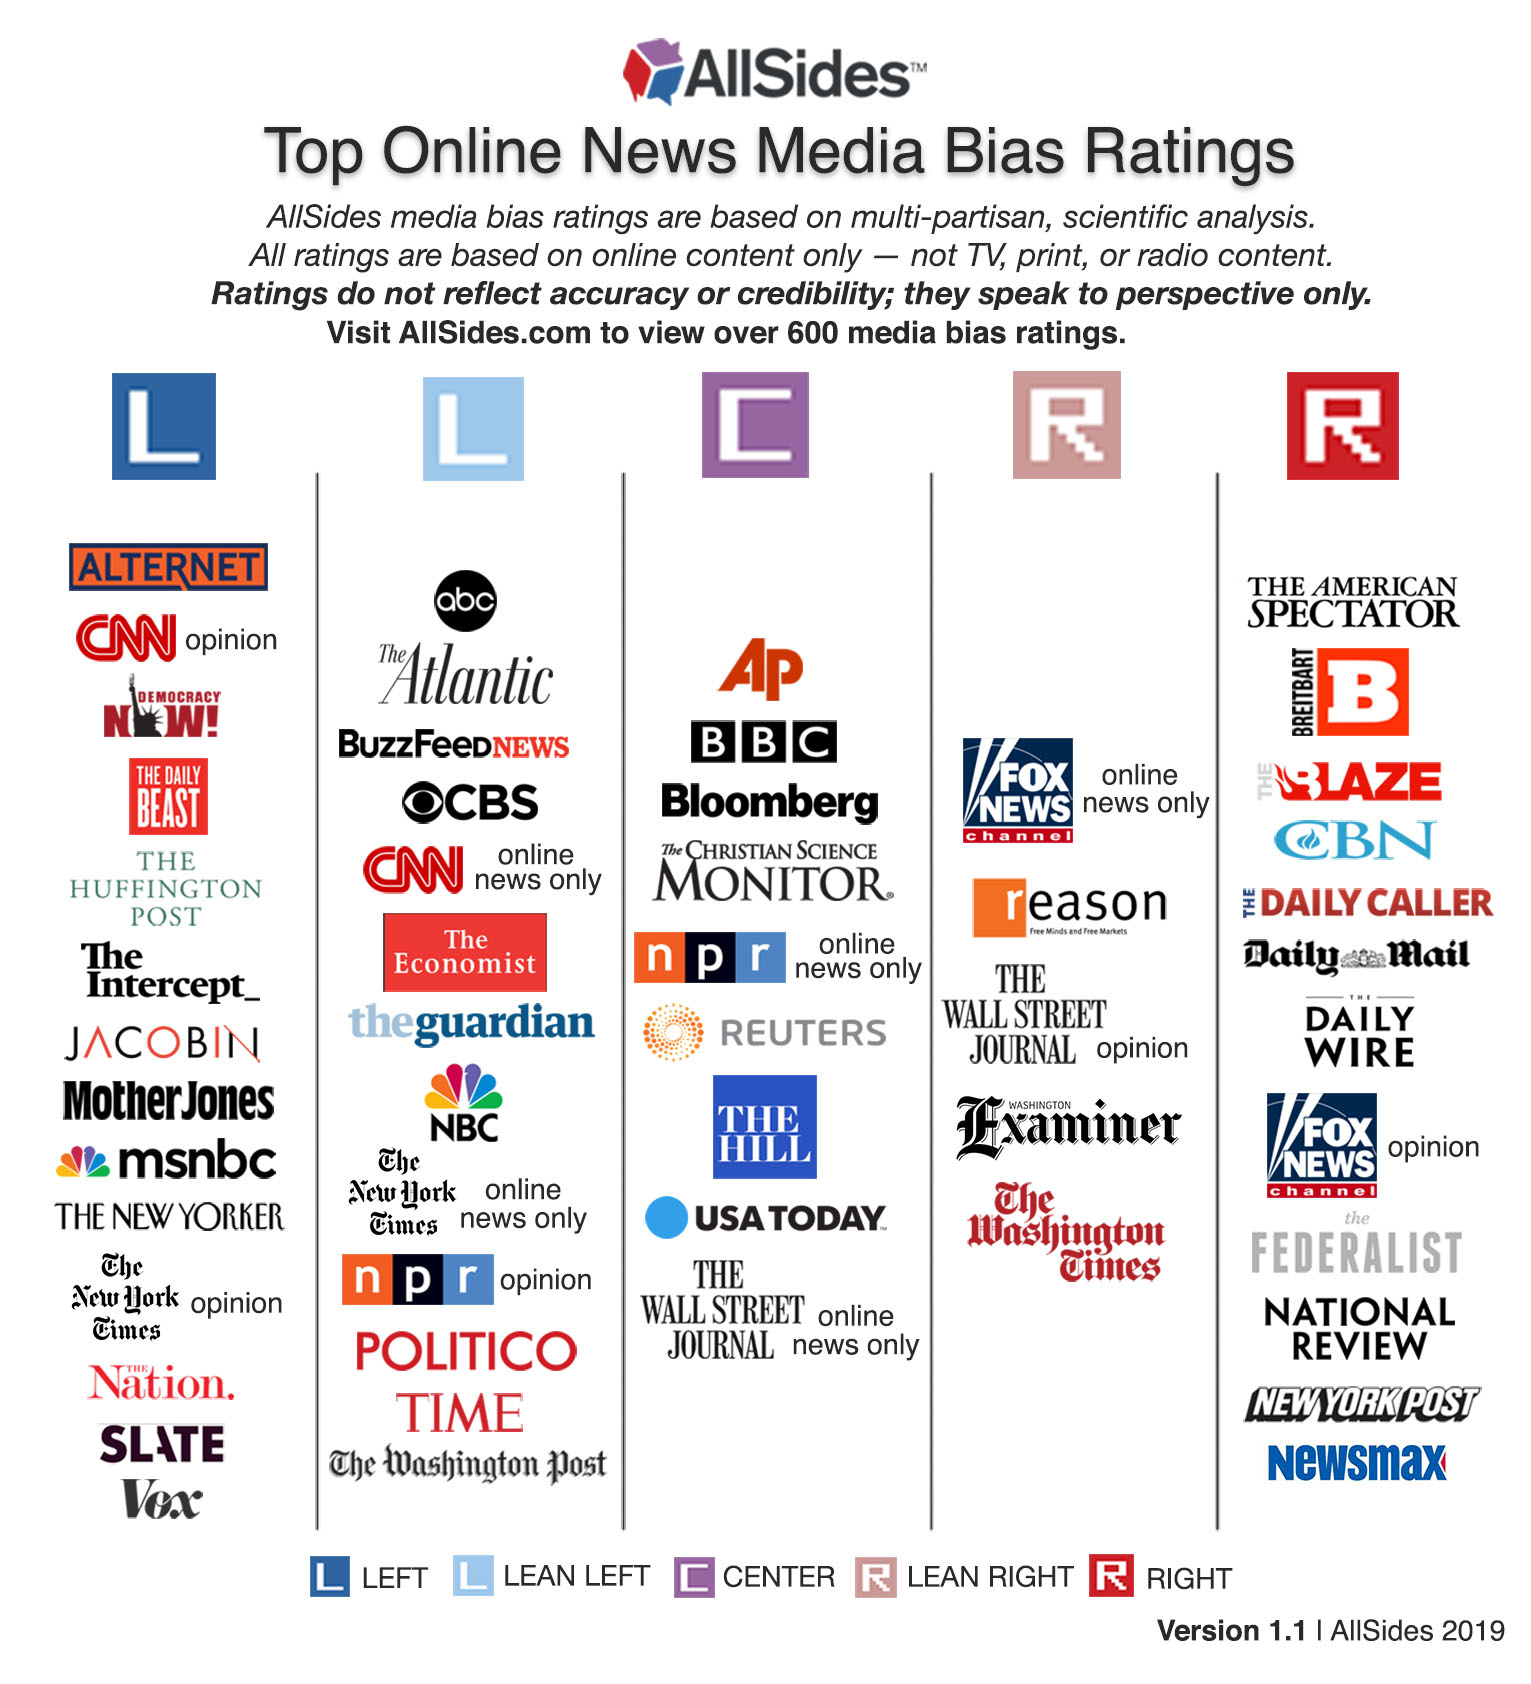
\includegraphics[width=\linewidth]{chapter1/figs/AllSidesMediaBiasChart}
	\caption[An example collection of News-Media sites that have been classified into biases; sourced from AllSides website.]{An example collection of News-Media sites that have been classified into biases; sourced from AllSides website~\cite{gable_media_2019}.}
	\label{fig:allsidesmediabiaschart}
\end{figure}
% </AllSides discussion>



% <sorting organisations>
A list of possible news sources was collected from AllSides on February 1st, 2019. In this collection was an organisation name, political bias, the number of user feedback ratings of the political bias, and, if available, the Twitter handles associated with the organisation. These collected news sources were broad, containing not just news-media organisations but authors, pundits and think tanks. 

We performed the following filtering: a source was only considered if it was a organisation (not an individual), that produced news content of a diverse range of topics. Many news sources were connected to think tanks or opinion groups, and only created news of a single topic or campaign. Further, if a news-media organisation has no Twitter account or had less than 10,000 followers it was removed from the pool. This mainly removed inactive organisations and local news organisations from small rural towns. 

Finally, a single source was removed as it was not in English (\emph{@univision}), and a single source (\emph{@theMRC}) was removed as its content was a subset of its sister site, CNSNews.  The result of this filtering process is 170 news-media organisations with associated Twitter accounts and categorised political biases.  A list of all news-media organisations under analysis can be seen in \autoref{sec:app_accounts} and all removed sources and the removal justification can be seen in \autoref{tab:app_removed_accounts}.
% </sorting organisations>

\subsubsection{Collection}
%  <Twitter collection>
Using the Twitter user handles associated with each news-media organisation, the history of all tweets for each account was collected using the Twitter application programming interface (API)\footnote{\url{https://developer.Twitter.com/en/docs}} and web-scraping tools\footnote{\url{https://github.com/twintproject/twint}}. Of interest in this work are the tweets each news organisation made between January 1st, 2019 to January 1st, 2020, which was the largest practical time-frame possible for analysis during this research project given data collection constraints. 

Over this period major news-media organisations tweeted pieces of news multiple times throughout the day. The manner in which each organisation does this can differ and no standard format is used. The tweets often come in the form of a single line description of an article, alongside a link to the article on the news-media organisation's website. The primary purpose of using social media sites to post these stories is to drive traffic to the organisation's website where they can earn revenue from ad impressions. As such, the format of such news tweets summarises core concepts from articles and frames them in their most essential and appealing way; often they are trying to create so-called `click-bait'~\cite{potthastCrowdsourcingLargeCorpus2018} but even standard reporting is often summarised in a clear tweet-length summary. This format is desirable for our work as we want to explore how the language news-media organisations use to appeal to consumers differs between organisations.

% breaking news
Twitter also serves as a tool for breaking news. The modern 24 hour news cycle has had many effects on journalism, including a pressure to produce breaking news at a lightning fast pace. The use of social media as a near instant tool for global public communication means that often no time is wasted in publishing a story, potentially while it is unfolding. Indeed, research has explored Twitter's role in breaking news in the cases of the 2011 UK summer riots~\cite{vis_Twitter_2013} through providing real time updates over the four days, and in the case of the death of Osama Bin Laden in 2011~\cite{hu_breaking_2012}, where the news was leaked and spread virally through social media before any news-media organisations could fully verify and publish stories on the claim. %
This rapid information exchange can prove dangerous, as in the case of the 2013 Boston Marathon bombing~\cite{starbird_rumors_2014}, where 29\% of the most viral content on Twitter was rumours and fake content~\cite{gupta_100_2013}.
% boston marathon
% These breaking news stories are sometimes, but not always, preceded by expressions such as ``\emph{Breaking News:}''. The inconsistent use of such a preamble can present challenge in our analysis of language moving forward, an \todo{will be explored more in this section}.
%  </Twitter collection>

\subsubsection{Account removal}
% <removal of inactive Twitter accounts>
Using this collection method a total of 3,221,769 tweets were collected from the 170 news-media organisation official Twitter accounts in the 2019 calendar year. This represents an average of above 50 tweets per day for each news organisation. However, the activity level and consistency of output vary greatly between organisations. \autoref{fig:data_cleaning_average_tweet_activity} shows the distribution of average daily number of tweets for each news-media organisations, showing that some news organisations produce very little content on average. This can be explained through two mechanisms.

\begin{figure}[!htbp]
	\centering
	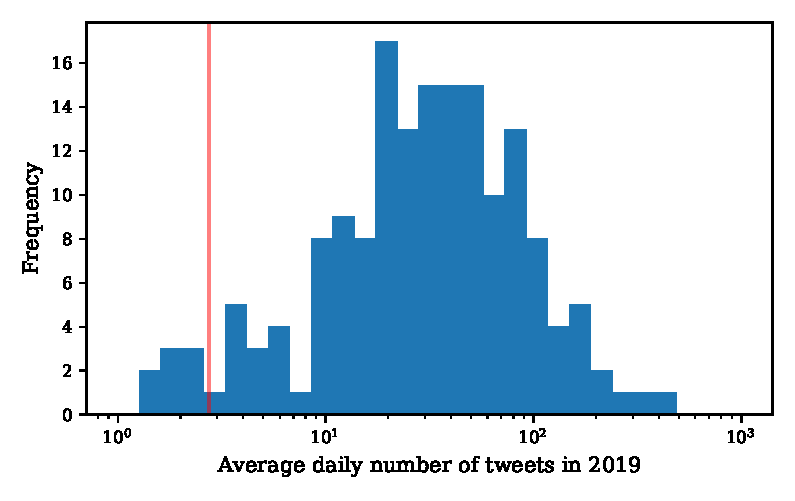
\includegraphics{chapter1/figs/averagetweetactivity}
	\caption{The average number of tweets produced each day during the 2019 calendar year for all 170 news-media organisations. The red line is the chosen threshold of 1000 tweets in the year, an average of 2.74 tweets per day.}
	\label{fig:data_cleaning_average_tweet_activity}
\end{figure}

Firstly, some organisations are not very active on social media. In particular, smaller organisations, which are typically less well resourced, place a lower priority on social media posting. This lower tweet volume presents a challenge for this work. In particular, the use of the non-parametric entropy estimator in \autoref{ch:crossentropy} requires a substantial amount of text to converge. Hence, organisations that produced less than 1000 tweets in 2019 were removed from further consideration. This removed a total of 11 news-media organisations, listed in  \autoref{tab:data_removed_low_tweet_counts}.


\begin{table}[!htbp]
	\centering
	\begin{tabular}{llr}
		\toprule
		News-media Organisation &    Bias  &  Number of tweets in 2019\\
		\midrule
		RealClearPolitics &      Center &  532 \\
		IJR  &  Lean Right &  777 \\
		WND News &         Right &  709 \\
		PRI &                Center &  346 \\
		EurekAlert! &            Center &  610 \\
		FAIR &     Center &  697 \\
		Crowdpac &            Center &  521 \\
		Inside Philanthropy &        Center &  781 \\
		Diplomatic Courier &         Center &  750 \\
		Peacock Panache &          Left &  198 \\
		Independent Voter &            Center &  303 \\
		\bottomrule
	\end{tabular}
\caption{Table of news-media organisations that were removed from data due to a low number of tweets in the 2019 calendar year.}
\label{tab:data_removed_low_tweet_counts}
\end{table}

Secondly, five news-media organisations, for reasons unknown, had large periods of time in which they did not post any tweets. These periods of time, spanning a few months, present key challenges to our investigation. 
Time is an important aspect of news, and this aspect is incorporated into our entropy estimation tools in \autoref{ch:crossentropy}. As such, news organisations that take long breaks will not have fair information theoretic comparisons. These five organisations, listed in \autoref{tab:data_removed_inactive_period} were removed from further analysis.

\begin{table}[!htbp]
	\centering
	\begin{tabular}{ll}
		\toprule
		News-media Organisation &    Bias \\
		\midrule
		American Thinker  &      Right \\
		Pacific Standard &  Lean Left \\
		Philly.com  &  Lean Left \\
		Splinter &       Left \\
		ThinkProgress  &       Left \\
		\bottomrule
	\end{tabular}
	\caption{Table of news-media organisations that were removed from data due to long periods of inactivity.}
	\label{tab:data_removed_inactive_period}
\end{table}


We examined the daily activity of each news-media organisation. An activity curve for the \emph{New York Times} can be seen in \autoref{fig:nytimes_and_tweets_by_weekday}(a). 
A clear weekly trend where tweet activity is decreased during the weekends is seen for most news-media organisations as exemplified when all news-media organisation tweets are aggregated in \autoref{fig:nytimes_and_tweets_by_weekday}(b). Further, many news-media organisations have distinct spikes at key points during the year. These spikes indicate an organisation is covering a rapidly-evolving, breaking news story, or responding to major changes in discourse through the day. These are interesting and important features in the data; the full collection of figures containing the daily activity levels of all included organisations can be seen in \autoref{app:activity}.

\begin{figure}[!htbp]
	\centering
	% \begin{subfigure}[t]{\textwidth}
	% 	\centering
	% 	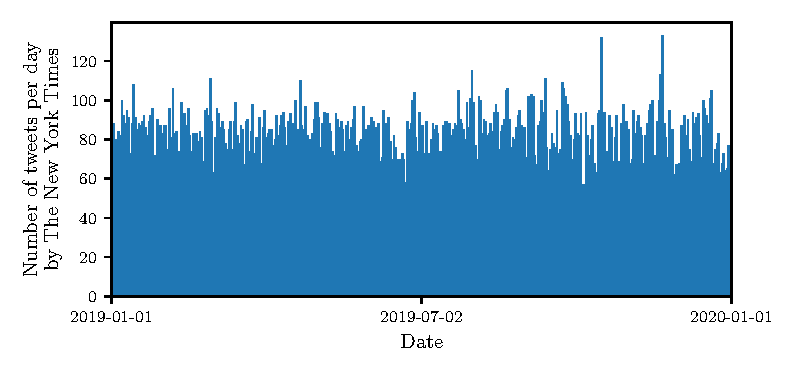
\includegraphics{chapter1/figs/tweet_times_nytimes.pdf}
	% 	\caption{}
	% 	\label{fig:data_newyorktime_activity}
	% \end{subfigure} 
	% \begin{subfigure}[t]{\textwidth}
	% 	\centering
	% 	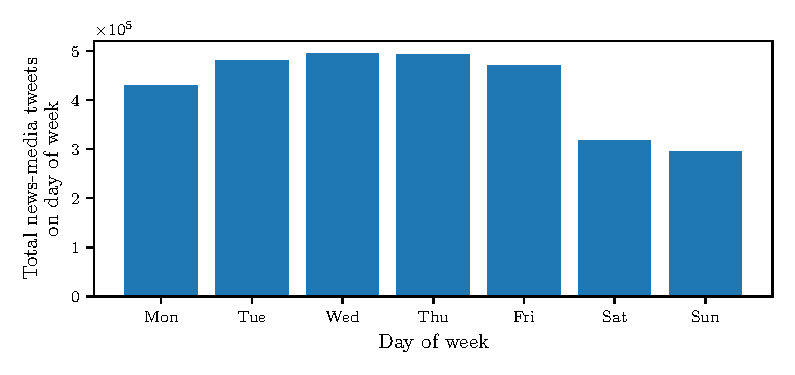
\includegraphics{chapter1/figs/tweet_by_weekday.pdf}
	% 	\caption{}
	% 	\label{fig:tweets_by_weekday}
	% \end{subfigure}
	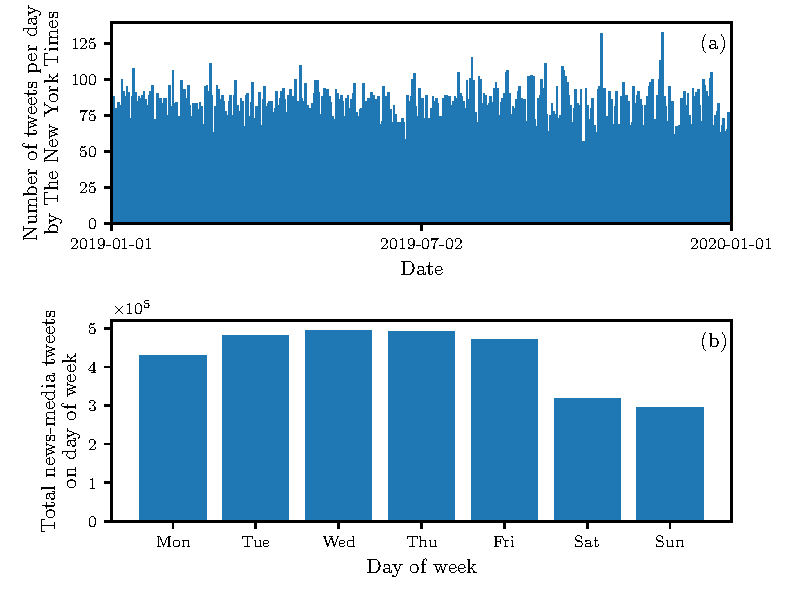
\includegraphics{chapter1/figs/nytimes_day_of_week_merge.pdf}
	\caption{News-media Twitter activity in 2019. (a) is activity for \emph{The New York Times} (account handle \emph{@nytimes}) which is the most followed news-media account with 44,800,317 followers and 31,029 tweets in 2019. Activity figures for other organisations are available in \autoref{app:activity}. (b) shows the total tweet counts by day of week the tweet was posted. A clear weekend reduction in content can be seen.}\label{fig:nytimes_and_tweets_by_weekday}
\end{figure}

% </removal of inactive Twitter accounts>

\subsubsection{Account analysis}
% <metadata>
After filtering we are left with 154 news-media organisations with complete data for the 2019 calendar year. %
These organisations average 52.97 tweets per day, with a total of 2,977,980 tweets.
% Of these organisations the bias distribution is still somewhat representative of social media. \ts{find a source that discusses why left wing is more popular on social media.} 
There are 73 organisations in the left half of the bias spectrum, 44 in the centre and 37 on the right (\autoref{fig:data_number_of_bias_organisations}). This distribution, although shifted towards the left, still provides sufficient samples of bias to explore further.

\begin{table}[!htbp]
	\centering
	\begin{tabular}{lr}
		\toprule
		Bias &   Number of Organisations \\
		\midrule
		{\color{Left} Left }&  31 \\
		{\color{LeanLeft} Lean Left }&  42 \\
		{\color{Center} Center }&  44 \\
		{\color{LeanRight} Lean Right }&  16 \\
		{\color{Right} Right }&  21 \\
		\bottomrule
	\end{tabular}
	\caption{The number of news-media organisations in each political bias classification in our data.}
	\label{fig:data_number_of_bias_organisations}
\end{table}

The news-media Twitter accounts also provide metadata about each organisation. Two useful pieces of metadata are the geographic location, and the number of followers on Twitter.

% location data
The Twitter account of each news-media organisation can elect to provide a free text `location'. In some cases this option can be used for other purposes, such for self promotion (\emph{e.g.} the \emph{New York Daily} states its location as `\texttt{New York City  /  fb.com/nydailynews}') and many organisations elected to leave the field blank. 
Of the organisations with text, locations can be difficult to disambiguate and compare. We therefore classified locations manually in \autoref{tab:data_locations}. Where multiple cities or locations are given, the largest possible inclusion was taken. For example `\texttt{New York and the World}' would become `Worldwide' in our classification, as would `\texttt{NYC, London, Paris, Hong Kong}'. There is a notable U.S focus to the data, as is expected using a U.S. based bias rating tool.

\begin{table}[!htbp]
	\centering
	\begin{tabular}{lr}
		\toprule
		Location &  Counts \\
		\midrule
		New York &      34 \\
		Washington, D.C. &      20 \\
		California &      11 \\
		Other US City &      44 \\
		General US &       8 \\
		Worldwide &       6 \\
		United Kingdom &       5 \\
		Qatar &       1 \\
		Pakistan &       1 \\
		Korea  &       1 \\
		Unspecified or Unclear &      43 \\
		\bottomrule
	\end{tabular}
	\caption{The aggregated self-defined locations of news-media organisations according to their Twitter account metadata. }
	\label{tab:data_locations}
\end{table}

% follower distributions
The number of followers a news-media organisation has on Twitter is an important metric, as it is a proxy for the `reach' of the account.

The most followed organisation in the dataset was the \emph{New York Times} with 44,800,317 accounts following it at the time of collection on the 13th January 2020. The least-followed account was \emph{CalMatters} with 15,069 followers. Interestingly, in addition to being more numerous, the follower counts were slightly higher for left biased organisations than for the right.  This is shown via the followers distributions for each bias in \autoref{fig:data_number_of_follow_by_bias_raincloud}, which is indicative of the larger trend in social media of slightly left-leaning demographics~\cite{mellonTwitterFacebookAre2017}.

\begin{figure}[!htbp]
	\centering
	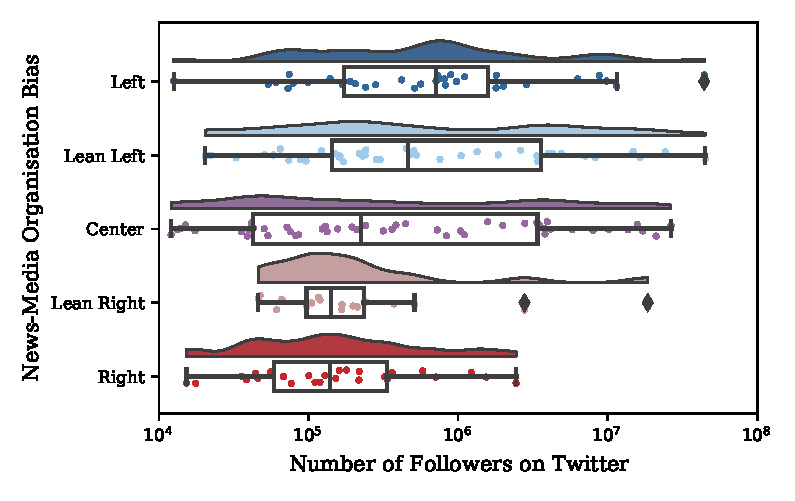
\includegraphics[width=\textwidth]{chapter1/figs/number_of_follow_by_bias_raincloud}
	\caption{Number of followers on Twitter of news-media organisations included in the data grouped according to political bias assigned by AllSides. The full range of political spectrum is represented in the data, with left leaning organisations having a higher average number of followers. }
	\label{fig:data_number_of_follow_by_bias_raincloud}
\end{figure}
% </metadata>

\subsection{Tokenization}

We process the 2,977,980 tweets from filtered dataset into an array of words. As discussed in \autoref{sec:tokenization}, the process of tokenization is applied to each string independently.

The TweetTokenizer\footnote{\url{www.nltk.org/api/nltk.tokenize}} from the Natural Language Toolkit (nltk) in Python is used. This built-in tokenizer is specially designed for tweet-style strings and bundles several useful features.

For each tweet, four steps are applied:
\begin{enumerate}
	\item Twitter account handles, which appear in the form `@account\_name', are removed. Across all accounts, these handles make up 0.88\% of the tokens. While some handles are contextual references, many are reference to piece authors. In the case of the \emph{Los Angeles Times}, 69\% of the references were to its own Twitter account. In general, these handles usually add uninformative differentiation between each organisation's description of the news, and make matching sub-sequences of tokens harder.
	\item Any sequence of a character that repeats more than three times is reduced to a maximum of 3. This has the effect of standardising text of similar meanings a common form, such as `waaaaayyyy' and `waaayyyyy' to `waaayyy'. In doing so, this reduction makes matches between these tokens far more likely.
	\item All URLs included in the text are removed. These URLs are almost always a link to an organisations own story associated with the tweet context. Many organisation's have multiple domains or sister-sites making these hard to isolate without removing all URLs.  
	\item The string is converted to lower-case and split at each white-space, giving an array of individual words. This creates the sequence of tokens that can be most easily compared between organisations.
\end{enumerate}

These steps are applied uniformly across the corpus to identify the flow of linguistic structure within news. In order to achieve this, we need to standardise the text to the most common possible format, such that text of similar phrasing and meaning will be matched between sources. These tokenization and text cleaning steps allow for these similarities to be expressed.


\subsubsection{Vocabulary sizes}\label{sec:vocabsizes}

With the tweets of each Twitter account tokenized, we can begin to explore the vocabulary sizes. The vocabulary size is the number of unique tokens that exist in the collection of all tweets from a news-media organisation, as introduced in \autoref{sec:background_vocab_sizes}. \autoref{fig:data_vocabvsactivity} shows the strong relationship between the amount of tweets produced and the number of unique words, with diminishing increases to vocabulary as new tweets are added.

The ratio of vocabulary size to number of tweets provides a first glimpse into the level of complexity in the language for each news-media organisation. Accounts that have a more specific focus/domain, such as political focused news (\emph{e.g.} \emph{The Hill}), increase their vocabulary at a slower rate as new tweets are added due to the consistently repeating domain specific words. In contrast, an account such as the \emph{The Guardian} produces a diverse array of content, and hence has a larger vocabulary size in contrast to its output.

We see the extreme variance in tweet activity reflected in the distribution of vocabulary size. The vocabulary sizes span from 2,976 unique tokens (\emph{ScienceDaily}) to 40,824 (\emph{The Guardian}). 

This presents a key challenge for this work. We need to find information flows between news-media organisations that can have content corpora that differ in size by two orders of magnitude, and vocabulary sizes that can differ by up to one. This can exacerbate the problems already presented by natural language, and informs the need to normalise flows in later sections.


\begin{figure}[!htbp]
\centering
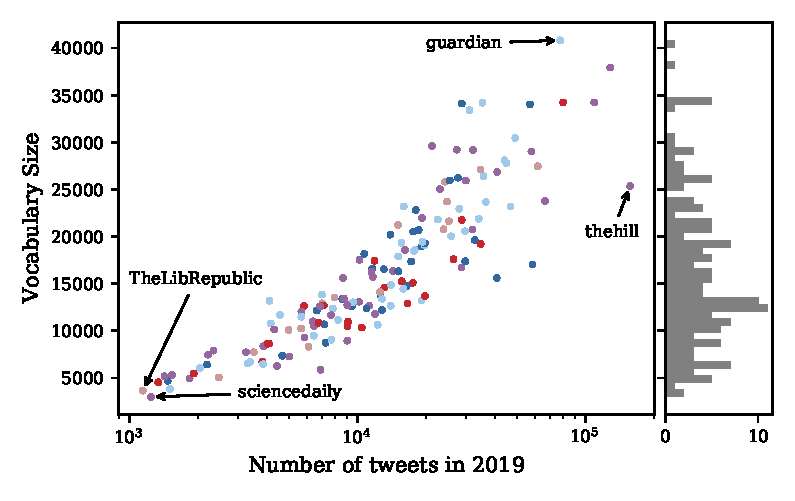
\includegraphics{chapter1/figs/vocab_vs_activity.pdf}
\caption{Vocabulary size from all tweets produced in 2019 for each news-media Twitter account and the total number of tweets produced.}\label{fig:data_vocabvsactivity}
\end{figure}

\subsection{Rank frequency distribution of vocabulary}\label{sec:zipf_fit}

In the remainder of this work we will often use this tokenized corpus of news-media tweets for our analysis. However, in some case we will want to generate synthetic text that has similar properties to our data here. As discussed in \autoref{sec:textgeneration}, we draw i.i.d. from a Zipf distribution to simulate such text. In order to match the properties of the data as best as possible, we fit a Zipf distribution to the data as show in \autoref{fig:data:fitted_zipf}. To extract the fitted scaling parameter of a Zipf distribution, we can fit a linear line to the log of each words frequency with the log of its frequency rank, in the corpus of all tweets. This fitting is meant to be approximate, as it is only used to inform the general range of Zipf law distributions used later, and the fitting of power-laws is often overdone~\cite{broidoScalefreeNetworksAre2019}. 

As has been seen in other corpora~\cite{williams_text_2015}, the rank-frequency distribution shows two different scaling regimes, where common words scale with $\alpha\approx 0.8$ and uncommon words scale with a much higher $\alpha \approx 2$, with an overall scaling parameter of $\alpha=1.2$. Later in thesis this we will use a variety of values for $\alpha$, usually in the range between $0.5$ and $2$.


\begin{figure}[!htbp]
\centering
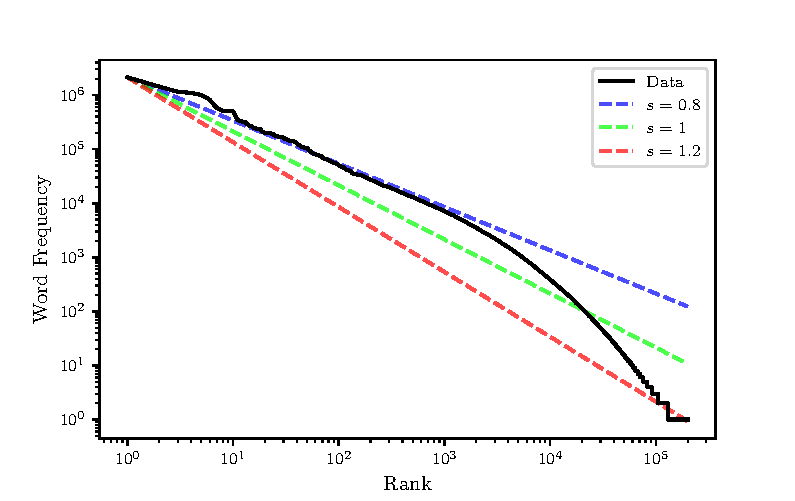
\includegraphics{chapter1/figs/fitted_zipf.pdf}
\caption{Word frequency of tokens in the corpus of all tweets produced by all news-media organisations compared the rank of the tokens by frequency. Zipf law distributions are also shown for varying scaling parameters, $\alpha$. \label{fig:data:fitted_zipf}}
\end{figure} 


Having now collected, cleaned, and performed a basic analysis of the data, we will now use it for two key purposes. Firstly, the development of the entropy estimation tools in \autoref{ch:crossentropy} and information flow measures in \autoref{ch:quotermodel} will use this dataset -- and the synthetic generation of text motivated by it -- to validate the techniques as reliable tools of information flow extraction. We then apply these tools to the data to produce a network, the analysis of which is discussed in \autoref{ch:ranking}.


%\the\textwidth
%
%% somewhere maybe summary
%60054638 words
